% ============================================================
% DIAGRAM: Generative Adversarial Network (2014)
% ============================================================
% Caption: Figure 5.2: GAN architecture with generator and discriminator.
%          (Adapted from Goodfellow et al., 2014, p. 2673)
% ============================================================

\documentclass[tikz,border=10pt]{standalone}
\usepackage{tikz}
\usepackage{amsmath}
\usepackage{amsfonts}

\usetikzlibrary{shapes,arrows,positioning,fit,calc,backgrounds}

\begin{document}

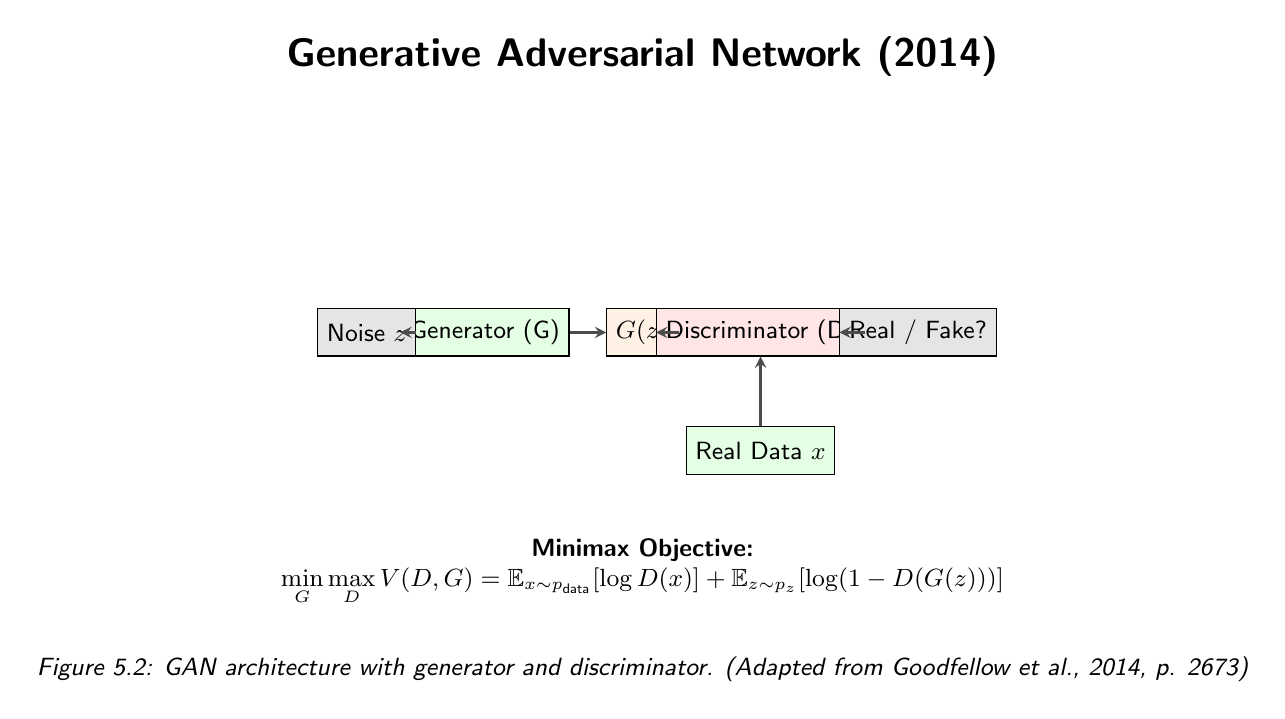
\begin{tikzpicture}[
    block/.style={draw, rectangle, minimum width=0.8cm, minimum height=0.6cm, fill=blue!10, font=\sffamily\small},
    edge/.style={-stealth, thick, draw=black!70},
    redge/.style={-stealth, thick, draw=red!70},
    label/.style={font=\sffamily\small},
    title/.style={font=\sffamily\Large\bfseries},
    caption/.style={font=\sffamily\small\itshape},
]

\node[title] at (0, 3.5) {Generative Adversarial Network (2014)};

% Generator
\node[block, fill=green!10] (gen) at (-2, 0) {Generator (G)};
\node[block, fill=gray!20] (noise) at (-3.5, 0) {Noise $z$};

% Generated samples
\node[block, fill=orange!10] (fake) at (0, 0) {$G(z)$};

% Real data
\node[block, fill=green!10] (real) at (1.5, -1.5) {Real Data $x$};

% Discriminator
\node[block, fill=red!10] (disc) at (1.5, 0) {Discriminator (D)};

% Output
\node[block, fill=gray!20] (out) at (3.5, 0) {Real / Fake?};

\draw[edge] (noise) -- (gen);
\draw[edge] (gen) -- (fake);
\draw[edge] (fake) -- (disc);
\draw[edge] (real) -- (disc);
\draw[edge] (disc) -- (out);

% Minimax
\node[align=center, font=\sffamily\small, anchor=north] at (0, -2.5) {
  \textbf{Minimax Objective:} \\
  $\displaystyle \min_G \max_D V(D,G) = \mathbb{E}_{x\sim p_{\text{data}}}[\log D(x)] + \mathbb{E}_{z\sim p_z}[\log(1-D(G(z)))]$
};

\node[caption, anchor=north] at (0, -4.0) {
  Figure 5.2: GAN architecture with generator and discriminator. (Adapted from Goodfellow et al., 2014, p. 2673)
};

\end{tikzpicture}
\end{document}
